En esta sección se expondrá la mayor cantidad de información sobre el desarrollo per se
del proyecto, desde la definición de requisitos y análisis inicial, hasta el proceso final
de testing y despliegue.

\section{Requisitos}

Definidos los objetivos del proyecto y tras realizar una primera reunión
con el tutor del TFG, se pueden definir de forma más concisa tanto los
requisitos funcionales como los no funcionales que debe cumplir la aplicación.

\subsection{Requisitos funcionales}

Una posible estructura de la memoria final asociada con cada TFG podría ser la siguiente (leed la normativa de TFG):\tutor{Esto se te ha colado ...}
\begin{itemize}
	\item RF1 Página de inicio - Debe existir una página principal que permita establecer el nombre dentro del juego al usuario,
	      que explique las reglas de juego y que establezca una interfaz sencilla para poder crear o unirse a una sala.
	\item RF2 Creación de salas - Un usuario debe ser capaz de crear una sala y también poder unirse a salas ya creadas mediante un
	      código único.
	\item RF3 Sala de juego y chat - Dentro de una sala, cada jugador debe poder visualizar a todos los jugadores con los que va a jugar
	      así como interactuar con ellos de forma sencilla mediante un chat.
	\item RF4 Empezar partida - Dado un número mínimo-máximo de jugadores uno de los jugadores debería tener la capacidad
	      para empezar una nueva partida.
	\item RF5 Conexiones - Tiene que existir una lógica que asuma conexiones o desconexiones accidentales y deliberadas por parte
	      de alguno o varios jugadores antes de empezar la partida en la sala, durante el juego o en la visualización de resultados.
	\item RF6 Inicio de partida - Al empezar la partida, el sistema debería proporcionar un orden aleatorio de turnos secuencial además de
	      la asignación de un rol junto a la contraseña a los jugadores Inocentes.
	\item RF7 Turnos - El orden secuencial a la hora de enviar palabras debería ser visible y destacar cuando es el turno
	      de un jugador en concreto.
	\item RF8 Enviar palabras - De forma secuencial, todos los jugadores deberían poder enviar una palabra semejante a la pista asumiendo
	      el juego de roles Outsider/Inocente sin interferencias por parte de otros jugadores.
	\item RF9 Votaciones - Al finalizar el envio de palabras se asume una fase de votaciones en la que, de forma asíncrona,
	      cada jugador vota a otro con el fin de acusarlo de Outsider y eliminarlo del juego.
	\item RF10 Resultados - Habiendo votado todos los usuarios, el sistema calcularía el resultado de esta votación para definir el
	      desenlace final de la ronda y se les mostraría a cada uno de los jugadores de forma simultánea este resultado.
	\item RF11 Gameloop - El sistema debe identificar cuando todos los jugadores han enviado sus palabras, mostrar la interfaz
	      de votación y finalmente gestionar y revelar los resultados a todos los jugadores de forma consistente.
	\item RF12 Varias\tutor{Múltiples} rondas - Si el número de jugadores  y el resultado de la ronda lo permite, el sistema debe asumir que tras
	      la finalización de una ronda pueden jugarse otras rondas de forma adicional si se desea. Por ejemplo, si hay cuatro jugadores y los tres jugadores
	      Inocentes no han identificado/votado al Outsider de forma correcta, se podría jugar otra ronda con tres jugadores si se ha votado de forma
	      errónea a un jugador Inocente o con los mismos cuatro si ha habido un empate en la votación.
	\item RF13 Varios Outsider - Si el número de jugadores es bastante alto, el sistema asignará el rol de Outsider a otro jugador de forma adicional.
	\item RF14 Última oportunidad - En el caso en el que el jugador con más votos sea el último Outsider en la partida, este tendrá un intento de
	      adivinar la contraseña que conocen los jugadores Inocentes.
	\item RF15 Multiplataforma - La aplicación debe ser accesible desde diferntes tipos de dispositivos como telefónos móviles u ordenadores portátiles
	      y de sobremesa.\tutor{Esto es un requisito no-funcional}
\end{itemize}

\subsection{Requisitos no funcionales}

\begin{itemize}
	\item RNF1 Usabilidad y accesibilidad básicas - La aplicación web debe atender a valores de usabilidad universales, como el uso del zoom o
	      el de diferentes resoluciones así como accesibilidad básica como el uso de colores con contraste por ejemplo.
	\item RNF2 Calidad de las conexiones - Se debe tener en cuenta la calidad y estabilidad de las conexiones mediante websocket para evitar
	      interrumpir, en la medida de lo posible, a los jugadores.
	\item RNF3 Información de estado - Se debe mantener informado al usuario del estado general de la partida así como de las posibles conexiones y desconexiones
	      por parte de otros jugadores.
	\item RNF4 Testing - El sistema tendrá una opción de desarrollo para poder ejecutar diversos tests que ponen
	      a prueba el correcto transcurso de una partida así como las conexiones y desconexiones en el entorno websocket del backend.
	\item RNF5 Despliegue y administración - La aplicación estará lsita para el despliegue y accesible para poder tener información de administración del servidor
	      backend.
	\item RNF6 Documentación - Todas las capacidades de administración actuales y de futuro desarrollo serán accesible de forma sencilla.
\end{itemize}

\section{Arquitectura general}

En este apartado, se pretende definir de forma más concisa la arquitectura software de la aplicación
teniendo en cuenta las tecnologías usadas y su interoperabilidad además del por qué se han tomado estas decisiones de diseño.

Después de haber analizado los diferentes requisitos y considerando las herramientas y conocimientos de partida,
se definen los servicios mínimos que debería ofrecer el sistema en conjunto:

\begin{enumerate}
	\item Backend - Django. Para empezar, es fundamental el uso de un servidor backend capaz de
	      gestionar la lógica de peticiones básica y que tenga capacidad para hacer uso de tecnología websocket.
	      Para esta tarea, se propone una implementación sencilla a través de Django. Se destaca que hay muy poca información que se
	      quiera tratar de forma persistente, por ello, no será necesario un servicio de base de datos adicional
	      y se recurrirá a la configuración por defecto de Django con un archivo SQLite.
	\item Servidor websocket - Redis (Django Channels). Al hacer uso de Django y de su particular implementación de
	      websockets, se ve indispensable el uso de un servicio adicional, un servidor redis. Este servidor es necesario para
	      poder hacer uso del sistema de 'capas', que permiten que varias instancias de controladores websocket
	      (denominados 'consumers') puedan comunicarse entre sí y con otras partes de Django \cite{djangoChannelsLayers}.
	\item Frontend - Vue3. Finalmente, solo quedaría gestionar la vista de la aplicación a través de Vue
	      que, para el desarrolador, facilita mucho el trabajo de frontend, integrando una gran cantidad de herramientas y componentes.
	      Dentro de este servicio se tendrá que trabajar la comunicación con el backend así como la visualización y lógica
	      web, por ejemplo, la lógica de navegación entre páginas a través de vue-router.
\end{enumerate}

Estos serían los elementos básicos del sistema, pero hay que tener en cuenta su
despliegue final. Para entenderlo todo de forma más organizada en la figura \ref{fig:res_arquitecturaSoftware} se muestra un esquema de la arquitectura
a nivel general. En el apéndice \tutor{referencia el apéndice} se muestra la misma imagen (\ref{fig:res_arquitecturaSoftware}) de mayor tamaño.

\begin{figure}[h]
	\centering
	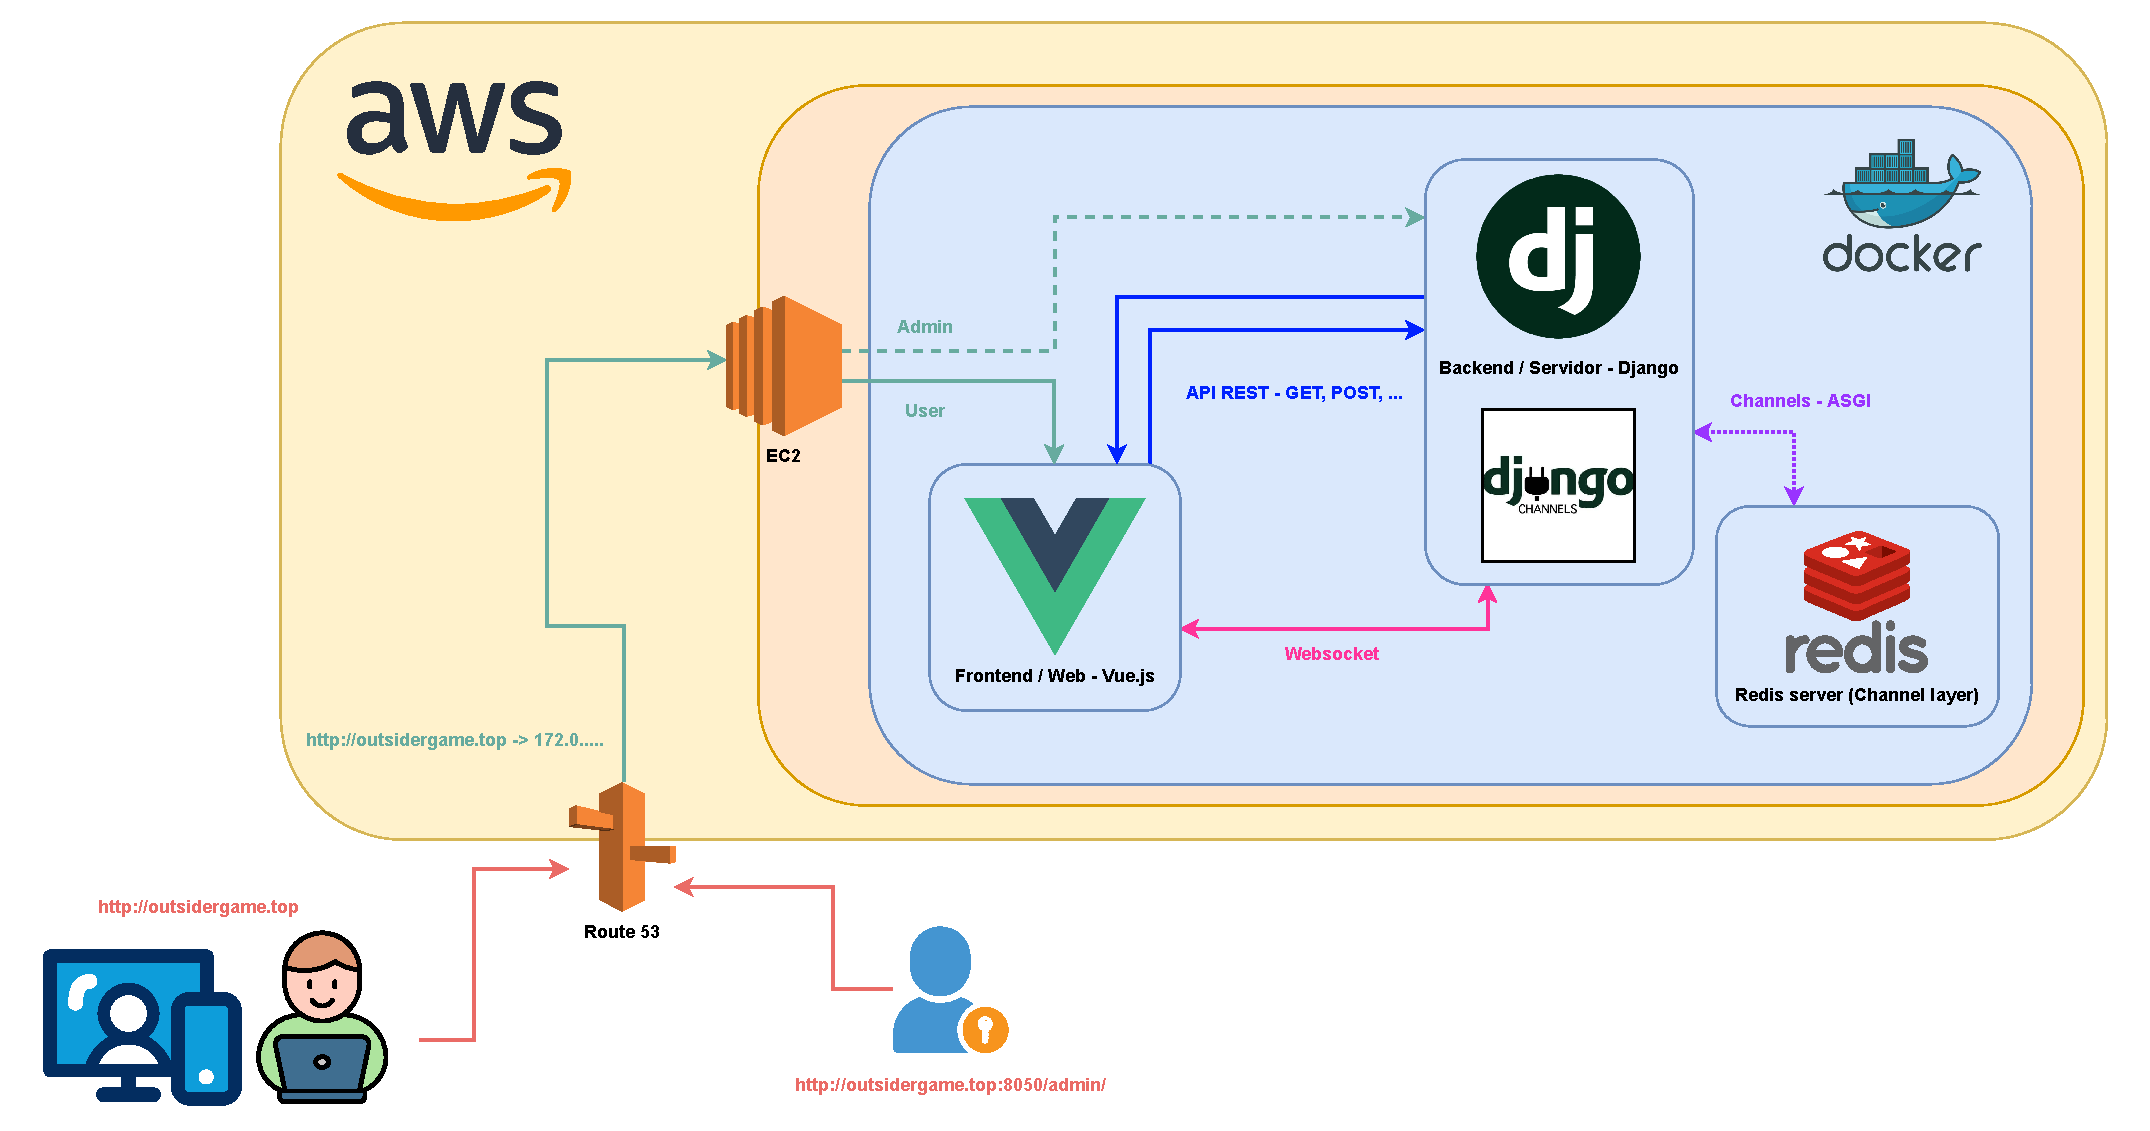
\includegraphics[width=\textwidth,clip=true]{res_arquitecturaSoftware.pdf}
	\caption{Arquitectura final del sistema}
	\label{fig:res_arquitecturaSoftware}
\end{figure}

De este esquema inicial cabría destacar un poco más en detalle el funcionamiento de las conexiones websocket, ya que, Django Channels 
está construido sobre la especificación ASGI (Asynchronous Server Gateway Interface), diseñada para proporcionar una interfaz estándar entre servidores web Python, frameworks y aplicaciones que soportan asincronía \cite{ASGI}. Dicho de otra forma,
permite hacer uso tanto de conexiones y peticiones HTTP como del uso del protocolo websocket sin problemas, algo totalmente nencesario para el desarrollo del proyecto. 

Dicho esto\tutor{Evita esta forma de comenzar las frases}, la comunicación a bajo nivel se hace un poco más enrevesada\tutor{suena un poco coloquial, mejor ``compleja''}, ya que, lo que facilita Django Channels son las herramientas de alto
nivel para trabajar directamente con los websockets. En la figura \ref{fig:res_esquemaDjangoChannels} se puede observar\tutor{detalla un poco lo que se observa en la figura, trata de describirlo} con mayor detalle como funcionan
las conexiones a bajo nivel en el entorno ASGI de Channels \cite{whatIsDjangoChannels}. De esta forma se puede entender un poco más sobre como funcionan las 
conexiones a bajo nivel respecto al anterior esquema general, el cual solo hace referencia a las conexiones de alto nivel entre los servicios principales de la aplicación.

\begin{figure}[h]
	\centering
	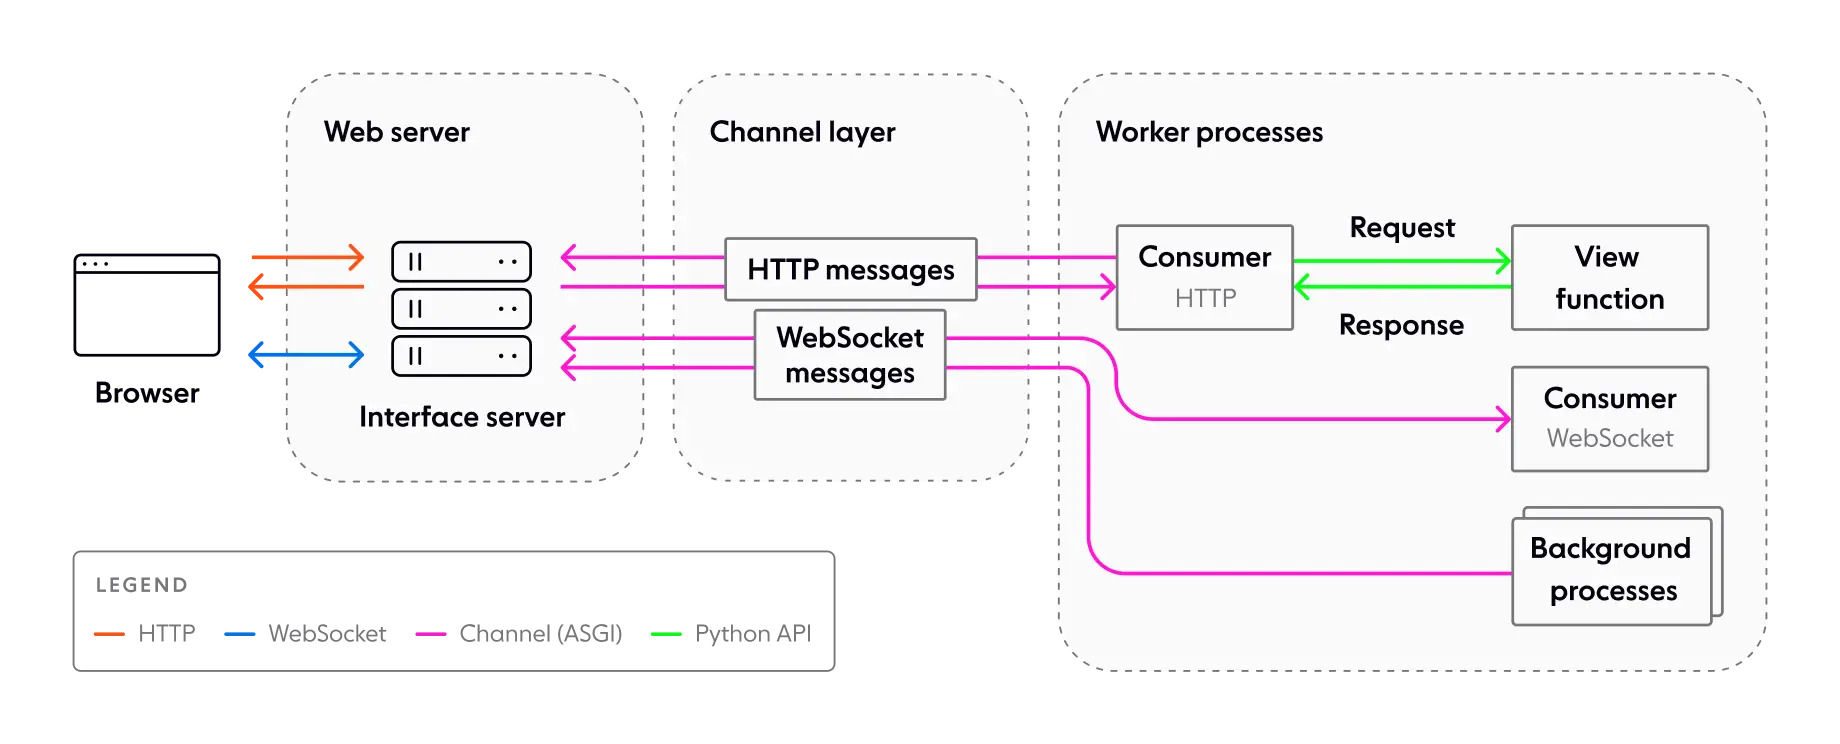
\includegraphics[width=\textwidth,clip=true]{res_esquemaDjangoChannels.jpg}
	\caption{Arquitectura de Django Channels}
	\label{fig:res_esquemaDjangoChannels}
\end{figure}

Obviando\tutor{Denostra tu trabajo decir que estás obviando parte de el. Como más arriba te pido que lo detalles, hila esta frase para referirte a que a partir de aquí hablas de aspectos de alto nivel} la comunicación ASGI a bajo nivel y los elementos asociados al despliegue (que se trataran con más detalle en las siguientes secciones), el resto del esquema es más sencillo: El usuario utilizará una URL, 
\href{http://outsidergame.top/}{outsidergame.top}  para acceder a la aplicación web y hacer uso de esta. La aplicación web (Vue) hará las necesarias comunicaciones (tanto HTTP como websocket) 
para acceder al contenido y la lógica del juego contenidas en el servidor de Django/Channels. De forma adicional se dispone una URL de administrador, 
\href{http://outsidergame.top:8050/admin/}{outsidergame.top:8050/admin/} protegida con credenciales para que el supuesto administrador de la web 
pueda gestionar algún dato de forma directa (principalmente la lista de palabras disponible).

\section{Diseño visual}

En una primera fase de conceptualización, se ha hecho uso de Figma \cite{figma} para calcular los tamaños y 
estructura general que deberían tener algunas de las páginas principales de la web. Se ha tenido en cuenta la disposición de los elementos cuandose está usando un dispositivo móvil o un
ordenador portatil (se entiende que funcione igual de bien en tablets y otros dispositivos similares), ya que, 
estos tienen diferentes proporciones de pantalla y hay pantallas que comprometen mucho la visualización en general.

En la figura \ref{fig:res_designLanding} se pueden observar a grandes rasgos los 
prototipados de la página principal y de la página de espera de juego con algunas notas además de colores 
y estilos provisionales.


\begin{figure}[h]													
	\begin{subfigure}{\textwidth}
		\centering
		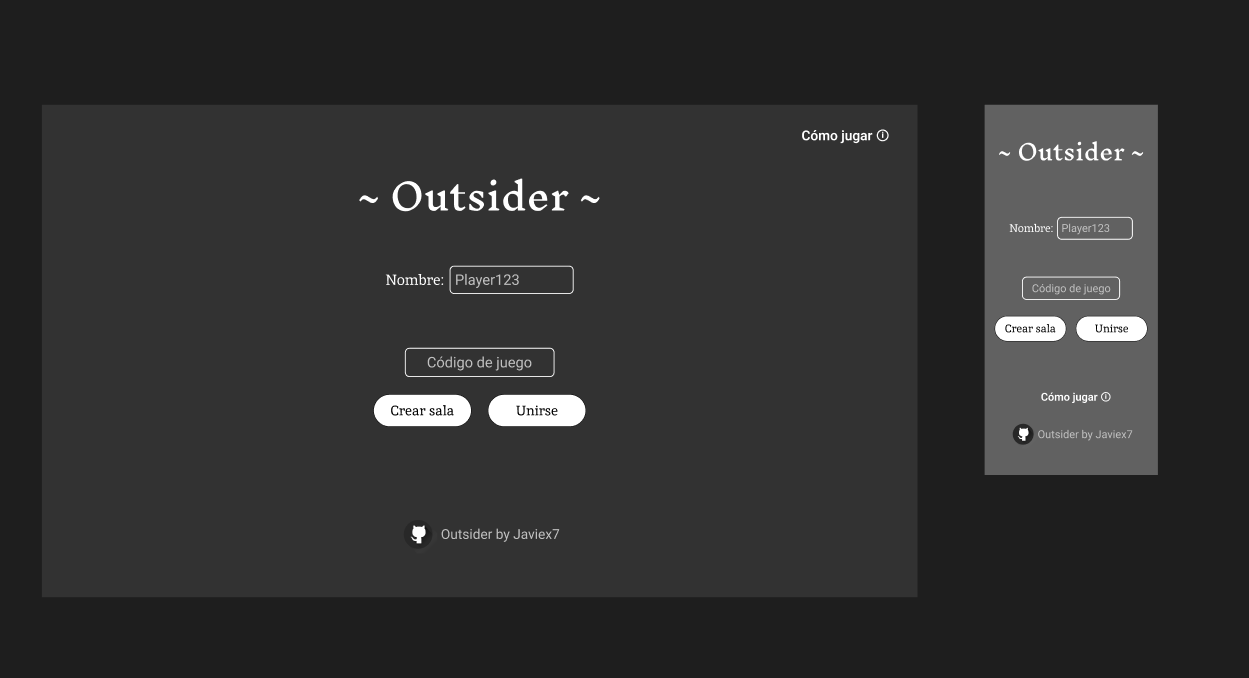
\includegraphics[height=7cm]{res_designLanding.png}
	\end{subfigure}
																																																																																																																																																																													
	\begin{subfigure}{\textwidth}
		\centering
		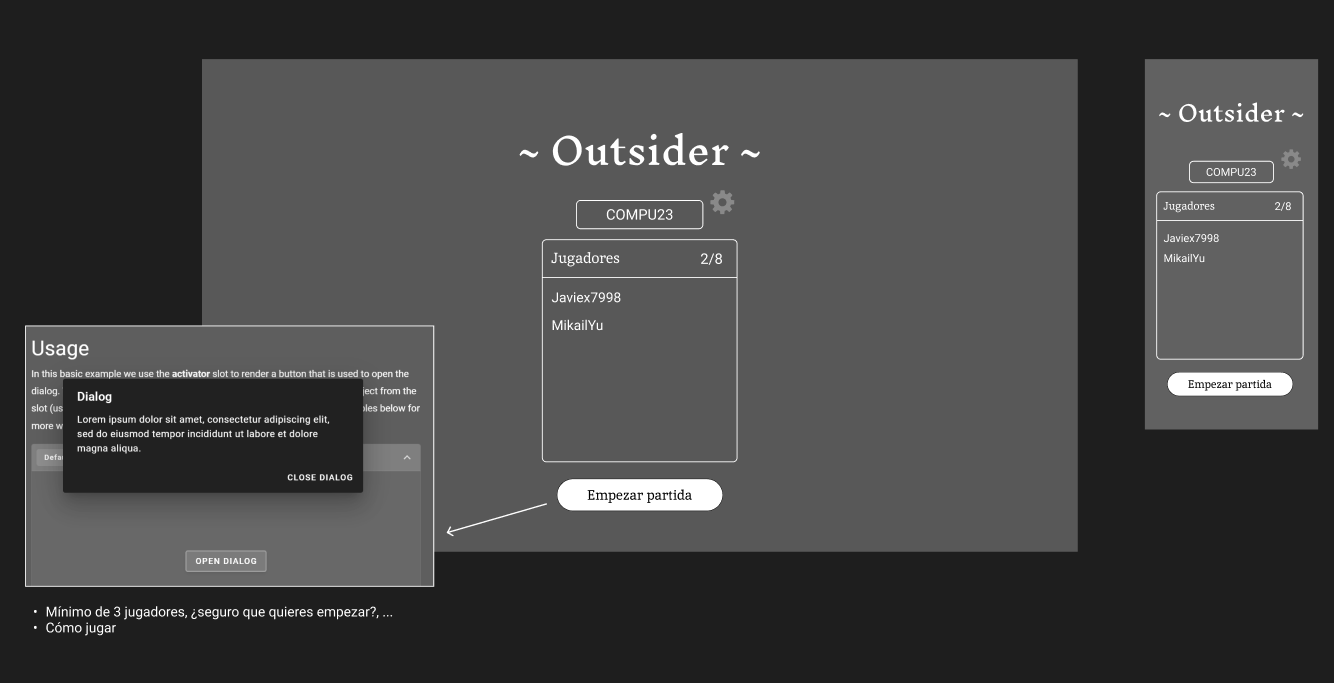
\includegraphics[height=7cm]{res_designLobby.png} 
	\end{subfigure}
																																																																																																																																																																																				
	\caption{Prototipados iniciales}
	\label{fig:res_designLanding}										
\end{figure}

Estos prototipos permiten concretar mejor el estilo y el diseño general de la página web. Además, 
se llevan a cabo varias pruebas de colores, tipografías y otros elementos estéticos antes de 
implementar estos estilos en la aplicación. En la figura \ref{fig:res_designJuego} se puede observar el primer diseño para la pantalla
de juego.

\begin{figure}[h]
	\centering
	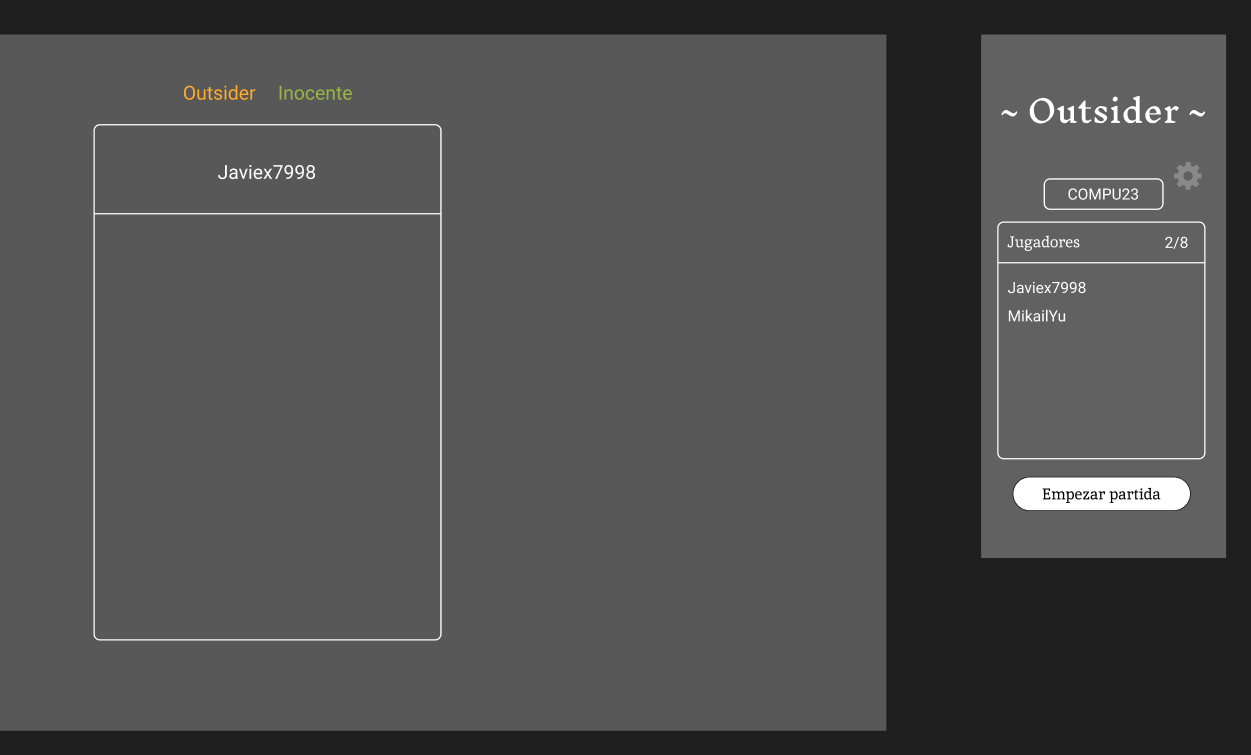
\includegraphics[height=7cm]{res_designJuego.png}
	\caption{Prototipo de la página de juego}
	\label{fig:res_designJuego}
\end{figure}

Cabría destacar que solo se ha tenido en cuenta la creación de unos pocos diseños debido a la facilidad de trabajar directamente
sobre los componentes de Vuetify y la necesidad de cambios constantes en la interfaz. De esta forma se ha evitado un 
sobreesfuerzo derivado de la iteración entre diseño e implementación.

\section{Implementación}

En esta sección se detallarán los aspectos más importantes para la implementación del sistema propuesto. 
Se abordarán tanto las funcionalidades y usos generales como los pequeños avances que se consideran significativos 
durante el proceso de desarrollo.

\subsection{Implementación básica Backend/Frontend}

La primera parte del desarrollo se ha basado en la implementación básica tanto del frontend a través de Vue como del 
backend con el uso de Django. Para esta tarea, lo más importante es la correcta instalación de dependencias así como de
la preparación del entorno de desarrollo.

Debido a la experencia previa en este apartado, no ha sido necesariamente complicado esta instalación inicial. Para Django,
la instalación es muy sencilla, solo se necesita tener python\tutor{alternas el uso de Python y python de manera poco consistente. Trata de usar siempre el término en mayúsculas} en el sistema y ejecutar un par de mandatos, por otra parte,
la instalación de Vue puede resultar algo más complicada, y en este caso se ha optado por hacer uso directamente de Vuetify para
tener todas las dependencias derivadas de Node.js integradas en el proyecto. De esta forma se debería tener\tutor{mejor: se tiene} una estructura de proyecto
como la que se puede observar en la figura \ref{fig:res_designJuego}. En el directorio 'outsider' se encuentran los archivos 
de configuración base de Django, mientras que en la carpeta 'outsider-front' se encuentra todo el código fuente relacionado 
con el uso de Vue/Vuetify. 

Se destaca que Django trabaja mediante el uso de 'aplicaciones'; haciendo referencia directa a la documentación de Django: 
El término 'aplicación' o 'app' describe un paquete de Python que proporciona un conjunto de funciones en concreto. 
Estas aplicaciones suelen incluir una combinación de modelos, vistas, 
plantillas, archivos estáticos, URLs y otras configuraciones relevantes a la aplicación en concreto \cite{django}. Debido a que 
la lógica estará enfocada principalmente a la gestión de las conexiones websocket, todos los modelos de datos y en general toda 
la lógica del backend Django estará contenida dentro del directorio 'logic'.

Como se había destacado antes, dentro de la carpeta 'outsider-front', se encontrará de forma bastante desglosada todos los componentes
que conforman el frontend de Vue así como todas las configuraciones y ficheros auxiliares pertinentes. En la sección \ref{Desarrollo del frontend}
se tratará en detalle la estructura del framework de Vue/Vuetify y la construcción de la página web (frontend).

De manera adicional, cabe destacar que, debido a las facilidades de mandatos que ofrecen los sistemas unix así como que el despliegue
final será en una maquina linux, se está trabajando a través de WSL, es decir,
ambas aplicaciones: frontend y backend, así como sus depedencias (python y node.js principalmente) se ejecutan en ubuntu a través de la interfaz
de WSL, ya que, el ordenador en el cual se está desarrolando el proyecto solo tiene instalado Windows 11 y por decisión propia se prefiere su uso de forma
cotidiana. Es importante tener esto en cuenta en primera instancia para evitar problemas en el futuro despliegue o mientras se está trabajando en el proyecto,
debido a que, el uso de mandatos y la disponiblidad de ciertos instaladores y librerías cambia drásticamente entre Windows y Linux.

Teniendo en cuenta esta instalación y configuración básica tanto del backend como del frontend, ya se puede trabajar directamente en el desarrollo de
la aplicación per se.

\subsection{Uso y aprendizaje de tecnologías websockets} 

Después de haber configurado el entorno de desarrollo base, cabría añadir los elementos necesarios para poder 
trabajar con tecnologías asíncronas.

Para el frontend solo será necesario hacer uso de la implementación del protocolo websocket \cite{websocketMDN}, mientras que en el 
backend, como ya se había comentado, será necesario hacer uso de otros elementos, en este caso, Django Channels. 
Por ello, lo primero será realizar la instalación de Channels en el server de Django.

Además de la instalación sencilla mediante pip install, es necesaria la configuración de varios settings del proyecto, así
como implementar el uso del servidor ASGI Daphne. En la documentación \cite{djangoChannelsInstall} se indica paso a paso el proceso 
de instalación en detalle si se quiere indagar en el tema\tutor{trata de dejar esto más formal}.

Con Django Channels\tutor{En otras partes de la memoria, has puesto channels en minúscula} instalado en el sistema, lo primero que se ha realizado son los propios tutoriales de uso, los cuales detallan 
la creación de un chat asíncrono, desde la configuración básica, hasta el uso de la funcionalidad de layers de forma asíncrona.

Estos tutoriales, que también se encuentran en la propia documentación de Channels \cite{djangoChannelsTutorial}, son 
de bastante calidad y se podrían comparar con la realización de una práctica guiada en una asignatura de la 
\escuelalargo. Se enseñan las capacidades básicas de los websocket y se va expandiendo a nivel funcional un ejemplo
de chat bastante completo. Se han encontrado tan interesantes estos ejemplos, que la funcionalidad backend del chat 
en la aplicación final, se ha dejado prácticamente como viene definida en estos tutoriales\tutor{mejor: se ha mantenido la configuración por defecto ...}.

En términos generales, el funcionamiento de Channels, vendría a ser la siguiente:

\begin{itemize}
	\item En primer lugar, después de tener el proyecto configurado y una aplicación de django\tutor{alternas mayúscula con minúcula al referirte a Django} lista para
	      trabajar con websockets (para este proyecto será la aplicación de 'logic'), será necesario la creación de un 
	      consumidor websocket.
	\item Cuando Django acepta una solicitud HTTP, consulta la configuración de url raíz para buscar una función de vista/view y luego 
	      llama a la función de vista para manejar la solicitud. De manera similar, cuando Channels acepta una conexión WebSocket, 
	      consulta la configuración de url para buscar un consumidor y luego llama a varias funciones dentro del propio consumidor 
	      para manejar eventos de la conexión.
	\item Siendo más específicos\tutor{estas enumerando, no puedes empezar un item así. La frase se entiende sin poner esta entradilla. Esto ocurre con los siguientes items de la lista, resulta confuso al leerlo}, los consumidores se estructuran en torno a una serie de métodos/funciones con nombre correspondientes al tipo de mensaje 
	      que recibe del propio websocket. En otras palabras, se tendrá un consumidor con un método 'connect', un método 'disconnect' y un método 'receive' 
	      que gestionarán o consumirán, valga la redundancia, los mensajes de tipo websocket de nueva conexión 'new WebSocket', los de desconexión 
	      'WebSocket.close()' y los de envío de mensajes estándar 'WebSocket.send()' respectivamente.
	\item De esta forma, se entiende que los mensajes generados en el frontend web a través de la conexión websocket se 'producen' con el objetivo
	      de que el backend 'consuma' estos mensajes mediante los propios 'consumidores' que se han instanciado a la hora de crear la comunicación websocket.
	\item Como inciso final\tutor{Por último ...}, el uso de Django Channels se basa en el uso de estos objetos consumidores de la forma que se vea 
	      más adecuada. Por ejemplo, cabe destacar que los consumidores pueden heredar de diferentes clases con diferentes características,
	      por ejemplo pueden exisitr consumidores síncronos, asíncronos, realizar decodificación JSON de forma automática, ...
\end{itemize}

Teniendo clara como funciona la lógica de consumidores, faltaría destacar la implementación propia que se ha diseñado para este proyecto: Debido a que 
la lógica gira en torno al control del flujo del juego, solo se hace uso de un controlador para gestionar la única conexión websocket que debería haber entre
un jugador y una sala de juego. Por esto útimo también se denomina al consumidor como 'RoomConsumer'. El código~\ref{alg:RoomConsumer} ejemplifica los métodos 
principales e inicialización del consumer en cuestión. Como se puede observar se ha hecho uso de un AsyncJsonWebsocketConsumer, con decodificación JSON y el uso de 
comunicación asíncrona para poder gestionar varias peticiones de forma paralela sin necesidad de esperar a que se completen las peticiones en orden.
\tutor{Corrige/reduce los espacios que se generan entre las lineas 10-11 y 11-12}
\begin{mypython}[float={h},caption={RoomConsumer},label={alg:RoomConsumer}]
	import json
	from channels.generic.websocket import AsyncJsonWebsocketConsumer
																																																	
	from .utils.consumer_classes import State, WebsocketUser
	from .utils import sync_rest_calls, consumer_methods
	
	class RoomConsumer(AsyncJsonWebsocketConsumer):
	def __init__(self, *args, **kwargs):
																																																	
	async def connect(self): \dots																																			
	async def disconnect(self, close_code):	\dots																																			
	async def receive_json(self, content): \dots	
\end{mypython}

De esta forma el servidor es capaz de trabajar con información que le llega desde el frontend, sin embargo es necesario la capacidad opuesta, el envío de información al 
frontend desde el propio servidor, es más, debido a la lógica del juego, se debería poder enviar información a varios clientes web. Por ejemplo, a la hora de empezar una partida
a nivel lógico en el servidor, se quiere indicar a todos los jugadores que están en la sala de que ha empezado la partida así como su rol y posible contraseña.

Para empezar, se debe hacer uso del sistema de layers ya que, es indispensable para diferenciar diferentes salas de juego y permitir 
la comunicación entre diferentes instancias de consumidores, en este caso, queremos que jugadores de una misma sala se comuniquen entre sí de forma constante. 
Por ello, además de gestionar el servidor redis mediante un contenedor docker (docker run --rm -p 6379:6379 redis:7\tutor{no es necesario indicar el comando aquí}), también se tiene que procesar toda la lógica de broadcast
o envio de mensajes desde el backend al frontend. Esto se realizará mediante el propio consumidor, el cual tiene la capacidad de suscribirse a un grupo haciendo uso
de la aplicación de layers. Esta última operación se debe realizar cuando se acepta una conexión websocket en el propio consumidor. 

En el código~\ref{alg:JoinGroup} se puede observar como se hace uso del método 'channel\textunderscore layer.group\textunderscore add()' para añadir al consumidor per se 
al grupo (siempre estará relacionado el grupo a nivel lógico con la sala de juego en la que esté el propio jugador) cuando se realiza una nueva conexión websocket (método connect del consumidor). 

\begin{mypython}[float={h},caption={Añadir consumer a un grupo},label={alg:JoinGroup}]
	async def connect(self):
		...
		# Join room group
		await self.channel_layer.group_add(self.room_group_name, self.channel_name)
		await self.accept()
									
\end{mypython}

Por otro lado, dentro del método receive, puede ser que un usuario en concreto decida enviar el mensaje para empezar la partida y su consumidor, además de hacer la lógica de juego, 
debe hacer uso del método 'channel\textunderscore layer.group\textunderscore send()' para que los diferentes consumidores que forman parte del mismo grupo reciban la 
información de que un jugador está intentando empezar un partida. 

Este mensaje se despachará\tutor{de nuevo, muy coloquial} en base al 'tipo' de mensaje que defina el propio método de broadcast, es decir debe
existir un método denominado como 'startGame' el cual, además de poder realizar lógica adicional (por ejemplo, solo enviar la contraseña a jugadores Inocentes) 
enviaría finalmente el mensaje de empezar partida desde el consumidor al propio websocket (el propio usuario en el cliente web) mediante el método 'send\textunderscore json()'. 

Se puede ver\tutor{apreciar} de forma resumida, tanto el código de broadcast como el envío del mensaje final al cliente en el código~\ref{alg:ReceiveCode}. Para otras acciones existirán
otros métodos correspondientes y en este código solo se resalta el uso de 'startGame' para ejemplificar el uso de grupos de consumers.

Para finalizar este apartado y haciendo un poco\tutor{de nuevo, muy coloquial} de resumen, el objeto consumidor, además de de gestionar los mensajes que le llegan desde el cliente web y procesar la lógica necesaria, 
es capaz de enviar nueva información de vuelta a usuarios que compartan un mismo grupo, que en el contexto de este proyecto serán las salas de juego. De esta forma se logra
una comunicación bidireccional usuario-servidor con la capacidad de poder relacionar de forma consistente un grupo de conexiones en concreto.

\begin{mypython}[float={h},caption={Broadcast a todos los consumidores y envío final al cliente},label={alg:ReceiveCode}]
						
	# RECEIVE: Websocket -> Consumer -> Consumer group
	async def receive_json(self, content):
		...	
		if action == "startGame":
		self = start_game
		message = {...}
		...	
		# GROUP: Consumer -> Consumer group
		await self.channel_layer.group_send(
		self.room_group_name,
		{"type": action, "message": message, "username": username},
		)
					
	# startGame: Consumer group -> Consumer -> WebSocket
	async def startGame(self, event):
		...
		# SEND: Consumer -> WebSocket
		await self.send_json(content={...})
									
\end{mypython}

\subsection{Implementación del backend}

\tutor{Esta sección es extraña, porque toda la subsección anterior también es backend. Para evitar que re-escribas todo, trata de darle un nombre más concreto a esta sección}
Habiendo explicado el funcionamiento general de Django Channels, se procede a definir en detalle los métodos y funcionalidades 
de la implementación de la lógica del juego, incluyendo elementos adicionales, como el uso de peticiones REST y teniendo en cuenta 
la legibilidad y estrucutra del código.

Para empezar, todo el código relevante que se va a tratar, pertenece a la aplicación de 'logic' dentro de la carpeta fuente del proyecto.
Dentro de esta carpeta destacamos los ficheros 'consumers.py' y 'viewsets.py'.

\begin{itemize}
	\item consumers.py - Teniendo en cuenta todo lo que se ha explicado en el apartado previo, dentro de 'consumers.py' se encuentra la lógica asociada
	 	  al consumidor websocket de la aplicación, RoomConsumer. Se destaca cada consumidor tiene una inicialización de datos que va a ir trabajando
		  a lo largo de la sesión. Estos datos debería estar sincronizados entre las diferentes instancias de consumer que pertenezcan 
		  al mismo grupo/sala, por ejemplo, la lista de jugadores Outsider o un flag booleano que indica el fin del juego. Además de estas variables el consumidor 
		  redefine con mucha lógica los métodos websocket básicos: connect, disconnect y receive (el receive se denomina json por heredar del tipo de consumidro 
		  AsyncJsonWebsocketConsumer). En el siguiente apartado se detallará la gestión de conexiones y desconexiones, pero por ahora, cabría destacar el método receive.

		  El método receive tendrá la mayor carga de lógica y es por eso que dentro de la carpeta utils (dentro de la aplicación de logic) se encontrarán
		  otros métodos auxiliares para separar mejor el código, ya que, el método receive funciona como un gran switch en base al mensaje que reciba el
		  consumidor desde websocket. Si un jugador envia el mensaje de siguiente turno (solo lo puede hacer el jugador cuyo turno este activo) el consumidor 
		  , además de gestionar la lógica pertinente para indicar que sería el turno del siguiente jugador (puede que se acabe la ronda por ejemplo), debe indicar
		  al resto de consumidores el resultado que haya sido calculado.

		  Para evitar acciones erróneas, existe una selección de acciones posibles, que serían: 'default', 'connection', 'startGame', 'nextTurn', 
		  'votingOutsider', 'lastChance', 'nextRound' y 'endGame' y estas hacen referencia a su traducción en español ('acción por defecto', 'conexión', 
		  'empezar juego', 'siguiente turno', 'votar outsider', 'última oportunidad', 'siguiente ronda' y 'final de juego'). Habiendo realizado la lógica de cada
		  acción, se le comunica al resto de consumidores la información pertinente y es por ello que se definen también todos los métodos que reciven la información
		  del grupo/sala con el mismo nombre de estas acciones. Por ejemplo, si la acción es 'votingOutsider', ese consumidor enviará un mensaje a todos los consumidores 
		  de su grupo de tipo 'votingOutsider', y cada uno de los consumidores ejecutará el método con el mismo nombre que el tipo de mensaje enviado por el consumidor original,
		  en este caso, será el método 'async def votingOutsider(self, event)'.

		  De forma extra, también se ha definido un Enum que identifica el estado de un jugador y una clase WebsocketUser que hace referencia a la información del usuario
		  que hace uso de la conexión websocket con el servidor a la hora de entrar en una sala de juego (dentro de 'utils/consumer\textunderscore classes.py'). De esta forma se 
		  facilita la lógica de la aplicación y se estructuran de forma más ordenada los datos.

	\item viewsets.py - Se está destacando muchas veces el hecho de 'entrar en una sala' por parte del usuario, pero esto no es una acción trivial, ya que, de alguna forma
		  el cliente web debería poder conocer de forma sencilla el estado de una supuesta sala si es que un usuario quiere crearla o en todo caso entrar a una. Es por ello, que se destaca la implementación
		  de una lógica basada en modelo de datos, es decir, el estado de las salas se define y actualiza en base de datos para poder gestionar de forma sencila las futuras conexiones websocket.

		  Esta lógica se realiza mediante Django estándar: Primero se definen modelos de datos, en este caso RoomModel, para guardar la información de estado de una sala/partida
		  y de forma adicional WordsListModel para definir una lista de palabras para el juego de forma persistente y fácilmente accesible. Definidos los modelos, simplemente se hace uso de ellos mediante
		  las vistas implementadas en 'viewsets.py'. Si un usuario quiere crear una sala, si no existe una sala con el mismo nombre, puede crearla sin problemas y ahora se puede gestionar sin problemas
		  la lógica websocket asociada, realizando una conexión inicial. De forma similar sin un usuario quiere entrar en una sala, se comprueba si existe para poder realizar realizar la conexión websocket.

		  Es importante destacar que se realizan peticiones a la base de datos desde el entorno asíncrono del consumidor websocket (desde 'consumers.py' 
		  y 'utils/consumer\textunderscore methods.py'), es por ello que dentro de la carpeta de utils también se define un fichero 'sync\textunderscore rest\textunderscore calls' que contiene 
		  los métodos de acceso a base de datos con un manejo específico (a través de la definición de un contexto síncrono y seguro) para que todo funcione sin problemas. Al final, es una necesidad
		  separar la lógica síncrona de la base de datos con la asíncrona de las comunicación con websockets.
	
\end{itemize}

De forma adicional destacamos la configuración básica de urls y enrutamiento, tanto para websocket (a través de 'routing.py') como para las vistas clásicas (en 'urls.py') así como de 
configuración adicional a la hora de iniciar o reiniciar el servidor backend (en 'apps.py'); esta configuración inicial se encarga de limpiar salas si se han eliminado 
de forma incorrecta debido a un bug del server o problemas de conexión mayores y, por otra parte, actualizar la lista de palabras que utiliza el juego cuando no se ha encontrado
una lista de palabras inicial válidas o se ha borrado de la base de datos en algún momento.


\subsection{Gestión de conexiones simultáneas y otros problemas generales}

\tutor{Si vas a hablar de problemas generales, trata de dar un título más genérico a esta subsección: ``Problemas afrontados durante el desarrollo'' o algo similar}	
En esta sección se destacan los principales problemas que se han ido encontrado a lo largo del desarrollo, especialmente los relacionados con 
la lógica en el backend.

\tutor{Separa los items que enumeras de otra forma. No se sabe de qué están hablando. Por ejemplo, puedes poner un título a cada item. El primero podría ser ``Problemas de sincronización''}
\begin{itemize}
	\item En primer lugar, es muy importante tener en cuenta problemas de sincronización como salas ya creadas, o códigos no válidos. A la hora de gestionar a varios jugadores en una misma sala
		  eran recurrentes los problemas relacioandos con la información que tiene un consumidor y otro, ya que, la mayor parte de la lógica, por ejemplo, calcular el resultado de una votación
		  es una tarea que solo debería realizar un consumidor en concretro que estuviese a la espera del resto de votaciones. Por ello, se trabajó mucho en la sincronización de información
		  entre todos los consumidores, así como en la creación de una lógica de listeners robusta en el frontend; siempre a la espera de nuevos mensajes websocket provenientes del servidor.
	
		  Por otra parte, se ideó un mecanismo clave en la gestión asíncrona de la lógica del juego: Hay muchos puntos en los cuales cualquier jugador podría empezar/acabar con la partida
		  o como se acaba de comentar, hay partes de código que solo tiene sentido que gestione un usuario/consumidor en exclusiva, para no repetir cálculos y respetar una sincronía dentro
		  de la comunicación asíncrona. Este tipo de problemas pueden resultar familiares a los que hayan trabajado con este tipo de tecnologías, personalmente\tutor{evita usar términos que se refieran a ti} se pensó en soluciones como el concepto de Barrier
		  a la hora de forzar la espera de un proceso en un punto hasta que el resto de procesos hayan llegado al mismo punto \cite{Barrier}. 
		
		  Finalmente, se llegó a una solución sencilla que también ayuda al diseño y experiencia de usuario: Un rol adicional de capitán o jefe de la sala. La clave radica en la sencillez de la idea, 
		  el primer jugador que entra en una sala (el creador) es el capitán de la sala, y eso le permite iniciar la partida y tener la capacidad de terminarla entre rondas. De esta forma, gran parte de lógica la asume el 
		  consumidor del websocket asociado al usuario capitán. El único problema es la posible desconexión de este capitán, por ello, una gran parte del desarrollo ha sido la correcta sincronización de conexiones dentro 
		  de la sala. Para evitar posibles problemas en la lógica del juego, si un jugador (que no ha sido eliminado y no está como espectador en el juego) se desconecta en mitad de partida, se cancela la partida 
		  y los jugadores vuelven a la página principal.
		
		  Esto es debido a que recalcular la lógica en mitad de partida se hace demasiado complicada, especialmente mostrar los cambios de forma visual y sencilla a los usuarios. Por otra parte, las partidas son
		  absurdamente\tutor{muy coloquial} rápidas y sencillas y se persigue un trato de la información sencillo y poco persistente. Solo exisite información de los usuarios mientras están en una sala de juego, si se cierra la página 
		  web no hay ninguna traza de información que se haya almacenado obviando el historial de navegación y los datos asociados a la caché del propio navegador.

	\item Dicho esto\tutor{de nuevo, evitamos comenzar así un item}, se querría\tutor{querría es un verbo que chirría en un texto académico} hablar también sobre la gestión de resultados de las rondas, ya que, también ha sido un apartado un poco tedioso. El juego funciona de forma sencila, pero con todas las reglas aplicadas
		  hay diversos resultados a la hora de tratar la información de votación de los jugadores, desde empates, hasta la imposibilidad de seguir jugando de forma coherente (mismo número de outsiders que de jugadores).
		  Por ende, es importante tener en cuenta lo complicado que se puede volver un simple diálogo de texto y tener en cuenta todos los resultados posibles. En este aspecto el testing automático puede facilitar las
		  cosas y por ello puede resultar bastante úitl aplicarlo desde un primer momento.

	\item Finalmente también se desearía discutir sobre un elemento menor: La lista de palabras. El juego debería proporcionar una lista de palabras para que los usuarios jueguen con las 
		  diversas contraseñas, de forma adicional, se ha querido poder modificar esa lista de palabras de forma sencilla mediante el administrador de Django y un campo JSON (en el apéndice se indicará en mayor detalle su uso).
		  Dicho esto, se ha ido modificando una regla que indica que se le debe proporcionar al jugador Outsider una 'contraseña falsa' si es el primer jugador en una ronda; esto es porque si 
		  no tiene ninguna clase de pista adicional, se hace complicado evitar ser descubierto como Outsider. Por ende, la lista de palabras se hace algo más compleja, ya que, en este caso, el Outsider
		  debería tener otra palabra que se parezca a nivel semántico a la contraseña, pero sin ser la propia contraseña; por ello, para generar esta lista de tuplas se ha hecho uso de ChatGPT \cite{ChatGPT} para
		  poder tener al menos unos datos iniciales con los que testear y mostrar la aplicación evitando palabras repetidas entre diferentes partidas. Igualmente esto sería un aspecto a mejorar e incluso
		  se podrían modificar las reglas para poder tratar con este aspecto en especial, porque, incluso haciendo uso de IA, se ha hecho muy poco consistente esta generación de tuplas de palabras semánticamente similares.
		
\end{itemize}


\subsection{Desarrollo del frontend} \label{Desarrollo del frontend}

Una vez explicado el desarrollo relacionado con el servidor/backend, se puede comenzar a abordar el desarrollo del frontend utilizando Vue
y las tecnologías web pertinentes. Para comenzar, todo el código del que se va a hablar se encuentro dentro de la carpeta 'outsider-front' dentro de la carpeta
principal del proyecto. Dentro de este directorio están los archivos específicos del proyecto (principalmente en la carpeta src), junto con las librerías de Node.js y otras 
configuraciones adicionales.

Vue solo hace una gran distinción entre elementos: páginas y componentes, que se distinguen por su uso específico. La diferencia es simplemente que 
las vistas son componentes con capacidad de enrutamiento; es decir, mientras que los componentes pueden actuar como bloques reutilizables de comportamiento, estilo 
y estructura en diversas partes de la página web, las vistas tienen una ruta específica dentro de la página web\tutor{trata de re-escribir esta última frase para clarificarla. Comienzas hablando de páginas y componentes pero lo primero que introduces son las vistas y las comparas con ... las vistas? algo se te ha colado aquí}. En el desarrollo del proyecto, como se pude observar 
en la siguiente figura (\ref{fig:res_estructFronted}), se han planteado dos vistas que definen la pagían de inicio y la página que gestiona la sala de juego. Por otra parte
existen diversos componentes reutilizables que se integran dentro de cada una de la vistas.

\begin{figure}[h]
	\centering
	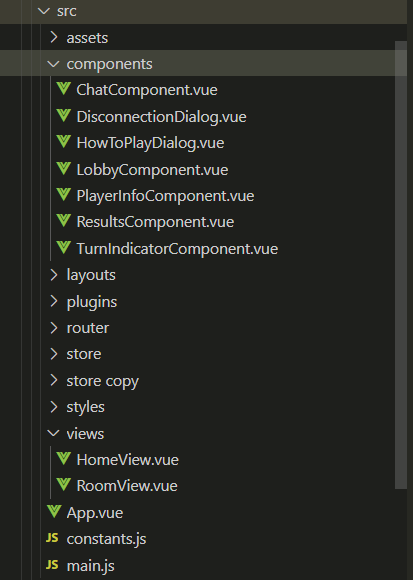
\includegraphics[height=10cm,clip=true]{res_estructFronted.png}
	\caption{Estructura de ficheros en el frontend}
	\label{fig:res_estructFronted}
\end{figure}

Antes de continuar con la descripción de las vistas, cabría destacar nuevamente el uso de Vuetify, ya que, se ha utlizado en gran medida para facilitar 
el trabajo de diseño y maquetación web. Esto se ha llevado a cabo principalmente mediante el uso de componentes de Vuetify; estos componentes de diferentes tipos, facilitan la
construcción de interfaz facilitando elementos como botones, carrouseles de elementos, menús, ... con la facilidad de cambiar su diseño de forma sencilla sin hacer uso
extensivo de CSS o en todo caso de código adicional para definir animaciones y comportamientos. De esta forma, se consigue una interfaz visualmente atractiva y de sencilla
creación.

Dicho esto, en la figura (\ref{fig:res_mainpage}) se puede observar la vista principal, 'HomeView.vue' en un dispositivo de escritorio. Es una vista muy sencilla y el código asociado no
es nada complejo, ya que solo tiene en cuenta la actuación de los botones para crear una sala y unirse a una sala mediante una petición sencilla al servidor con el uso de axios \cite{vueAxios}. 
Se tiene en cuenta que el nombre de usuario no sea ni demasiado corto, ni demasiado largo así como que el código de sala esté presente a la hora de intentar acceder a una sala de juego 
(o intentar crearla). También se proporcionan mensajes de 'error' si ha habido alguna incidencia (normalmente el intertar unirse a una sala que no existe o al intentar crear una sala ya existente). 
Para finalizar, la página también muestra con mucho detalle un diálogo con todas las instrucciones del juego si se pulsa el botón de 'Cómo jugar'.

\begin{figure}[h]
	\centering
	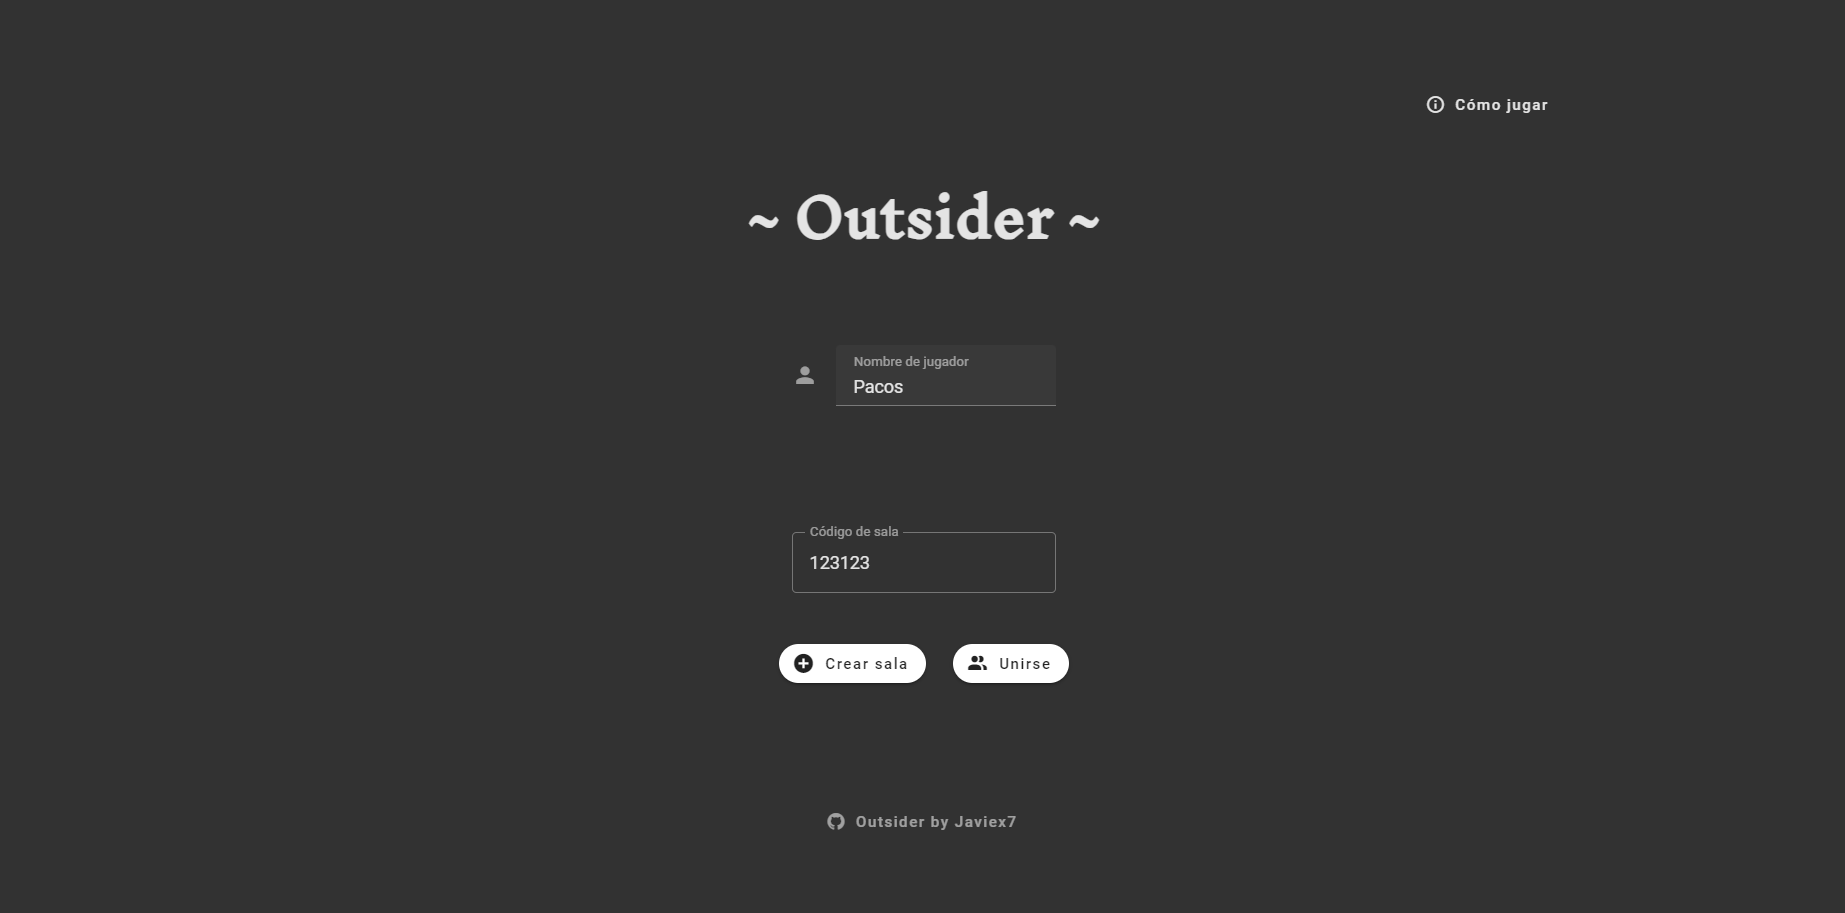
\includegraphics[width=\textwidth,clip=true]{res_mainpage.png}
	\caption{Página principal}
	\label{fig:res_mainpage}
\end{figure}

La otra vista, 'RoomView.vue', bastante más compleja, maneja toda la interfaz gráfica así como la lógica de peticiones websocket asociadas al juego per se, desde la
visualización y funcionamiento del chat, hasta la correcta presentación de los resultados de una ronda.

Para empezar, destacamos el LobbyComponent, encargado de mostrar y gestionar, dentro de la vista de la sala todos los elementos relacionados con la sala de espera, etre los que se
incluye un chat entre los miembros actuales de la sala, diferentes indicadores del estado de la sala (código de sala para que se puedan unir otros usuarios, número de jugadores y
lista con indicadores sobre capitanía de la sala) y un botón que sirve para iniciar la partida por parte del capitán de la sala si hay más de dos usuarios presentes.

En la figura (\ref{fig:res_lobby}) se puede ver un lobby/sala de dos jugadores interactuando con el chat así como otra sala con seis jugadores listos para jugar. De esta sección solo
cabría resaltar que se indica cuando se jugará con un outsider adicional (con seis o más jugadores) y también que, al lado de cada nombre de usuario se indica quién es el capitán mediante
un logo de corona y resaltado en azul además de quién es el propio usuario que está haciendo uso de la aplicación mediante otro icono de cuenta/usuario al lado del nombre introducido
antes de ingresar en la sala.

\begin{figure}[h]
   \centering
   \begin{minipage}{0.45\textwidth}
	\centering
	  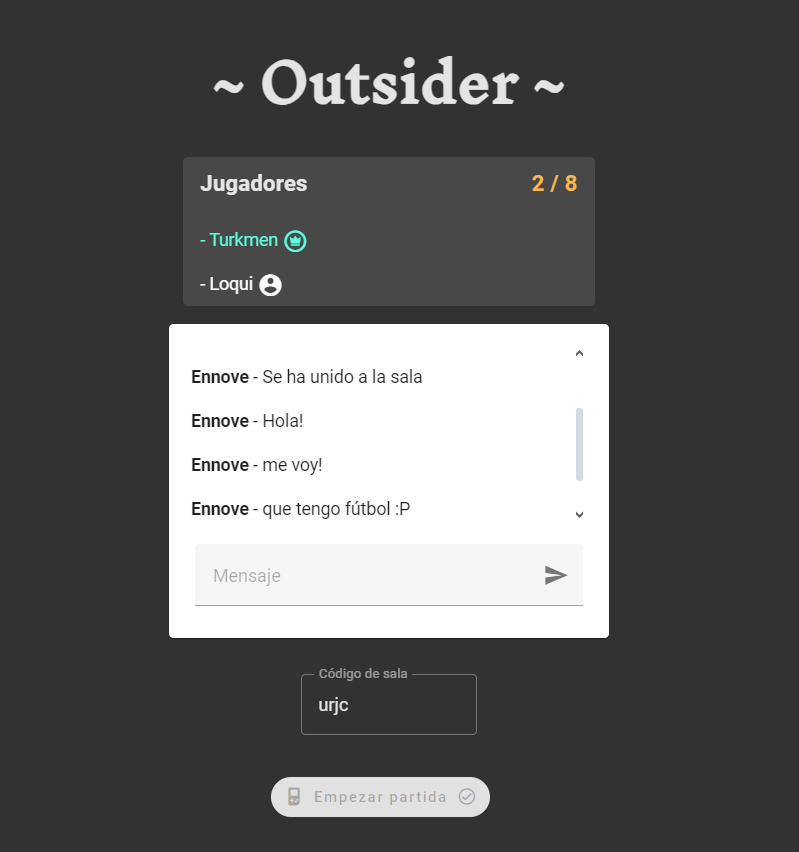
\includegraphics[clip=true,width=\textwidth]{res_lobby2.png}\\
   \end{minipage}
   \hfill
   \begin{minipage}{0.45\textwidth}
	\centering
	  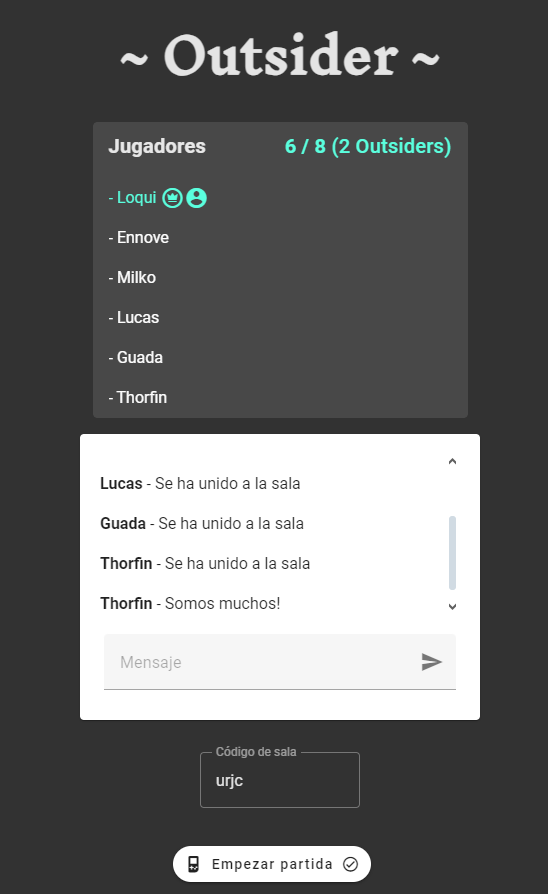
\includegraphics[clip=true,width=\textwidth]{res_lobby1.png}\\
   \end{minipage}
   \caption{Sala de espera con diferentes números de usuarios}
   \label{fig:res_lobby}
 \end{figure}

\section{Testing}
\tutor{Mejor: Pruebas automáticas}

\section{Pruebas con usuarios}
\tutor{Mejor: Pruebas manuales. Ya después puedes hablar de pruebas con usuarios en esta misma sección}

\section{Despliegue}

\tutor{Entiendo que simplemente no has llegado aquí}





